% !TeX root = ../Harte_Kugeln.tex
\section{Methode }
%\TODO[überschriften vllt anpassen]
Harte Kugeln sind ein vereinfachtes Modell für die Interaktion zwischen Molekülen, bei der angenommen wird, dass Moleküle runde Objekte (Kugeln) sind, welche nur durch elastische Stöße miteinander wechselwirken.
Dass die Stöße elastisch sind, bedeutet, dass keine Energie durch Zustandsänderung der Kugeln zugeführt wird oder verloren geht. Es findet also weder Deformation noch Erwärmung der Kugeln statt und auch der Drehimpuls spielt keine Rolle. Die Kugeln bewegen sich daher frei mit konstantem Impuls und konstanter Energie, bis sie auf eine andere Kugel -- oder bei nicht periodischen Randbedingungen auf die Grenze der Simulation -- stoßen. Das Potential eines derartigen Moleküls ist in Abb. \ref{fig:hkpotential} dargestellt.
\begin{figure}[H] \centering
\begin{tikzpicture}
	\begin{axis}[
		xlabel=$r$,
		xtick={0,2,8},
		 xticklabels={$0$,$R$,$\infty$},
		 ytick={0,10},
		 yticklabels={$0$,$\infty$},
		ylabel={$U(r)$}
	]
%\addplot+[color=blue,thick] coordinates { (0,2) (2,2)  (2,0) (9,0) }; % + wegmachen wenn punkte stören
\addplot[color=red] coordinates { (0,10) (2,10) (2,10) (2,0) (8,0) };    % auskommentieren je nachdem welcher plot besser ist (ggfs Achse anpassen)
\end{axis}
\end{tikzpicture}
\caption{Potential einer harten Kugel mit Radius $R$ auf Punktladungen im Abstand $r$}
 \label{fig:hkpotential}
\end{figure} 
\subsection{Ereignisbasierte Molekulardynamik}

Im Gegensatz zur herkömmlichen Molekulardynamik, bei der die Bewegung der Moleküle aus Integration der wirkenden Kräfte mit einem konstanten Zeitschritt folgt, wird bei der ereignisbasierten Molekulardynamik eine Liste über alle (zumindest alle relevanten) in der Zukunft liegenden Stöße geführt. Nach jedem Stoß wird die Zeit bis zum nächsten Stoß ``vorgespult'', diese Kollision berechnet und die Liste aktualisiert.

%Das untersuchte System war eine Box mit periodischen Randbedingungen gefüllt mit harten Kugeln (\ref{sec:hk})

Die Motivation der Methode ist, dass bei herkömmlicher MD (Molekulardynamik) mit konstantem Zeitschritt bei der Simulation harter Kugeln zwischen zwei Stößen viele unnötige Berechnungen durchgeführt werden. Wenn man den Zeitschritt größer macht, würde sich diese Anzahl zwar senken, dafür hätte man bei Stößen das Problem, dass sich eine Kugel innerhalb eines Zeitschritts in eine andere hinein bewegen könnte, was dann entweder zu Ungenauigkeiten oder zusätzlichem Rechenaufwand (Zeit zurück drehen und mit kleineren Zeitschritten sondieren) führt.
% erweitern?

\subsection{Berechnung der Stöße}
\newcommand{\reffig}[1]{Abbildung \ref{fig:#1}}

Um die nächste Stoßzeit zu ermitteln, genügt es, sich jeweils zwei Kugeln anzusehen und deren Kollisionszeit zu berechnen. Weiß man die Kollisionszeiten aller Kugeln im System, so weiß man auch den Zeitpunkt der nächsten Kollision. Man muss also nicht das System als ganzes betrachten, es genügt das Verhalten von jeweils zwei Kugeln zu kennen.
Im Zentrum der Simulation steht somit der Algorithmus zur Erkennung, ob und wann zwei Kugeln einander stoßen werden. 
Da wir eine Box mit periodischen Randbedingungen betrachten, muss der gewählte Algorithmus auch mit Kugeln am Rand der Box klarkommen. Unser Ansatz beruht auf einer Koordinatentransformation und wird in diesem Kapitel näher beschrieben.


% !TeX root = ../Harte_Kugeln.tex
\subsubsection{Kollisionsprüfung} % Probenentnahme? Messungsintervalle? 

%Parameter zur Darstellung der Box und Kugeln in diesem Absatz
\newcommand{\BoxW}{10}
\newcommand{\BoxH}{7}
\newcommand{\Kradius}{.7}

\newcommand{\Kx}{7}
\newcommand{\Ky}{6}

\newcommand{\vxa}{6/3}
\newcommand{\vya}{2/3}
\newcommand{\vxb}{-5/3}
\newcommand{\vyb}{3/3}

\newcommand{\Dx}{-2.5}
\newcommand{\Dy}{-5}

\newcommand{\BoxC}{\BoxW / 2 , \BoxH / 2}
\newcommand{\BoxWh}{\BoxW / 2}
\newcommand{\BoxHh}{\BoxH / 2}

\newcommand{\drawKugel}[1]{
    \draw[fill=black] 	(#1) circle (0.15em);
    \draw		(#1) circle (\Kradius);
}

\newcommand{\dis}{r_{21}}
\newcommand{\vdis}{\vec{r}_{21}}
\newcommand{\vdissq}{\left|\vdis\right|^2}

\newcommand{\vel}{v_{21}}
\newcommand{\vvel}{\vec{v}_{21}}
\newcommand{\vvelsq}{\left|\vvel\right|^2}
\newcommand{\dia}{d}

%\subsubsection{Koordinatentransformation}
Zur besseren Veranschaulichung wird der Algorithmus in 2 Dimensionen vorgestellt, er ist jedoch ohne Probleme auf beliebige Dimensionen erweiterbar.\\
In \reffig{Koortrans01} ist die Ausgangsposition zweier beliebiger Kugeln dargestellt. In dieser Darstellung ist eine Berechnung der Kollision erschwert da beide Kugeln ohne Kontakt und zu verschiedenen Zeiten die betrachtete Box verlassen.

% !TeX root = ../Harte_Kugeln.tex

\begin{figure}[H]
  \centering
  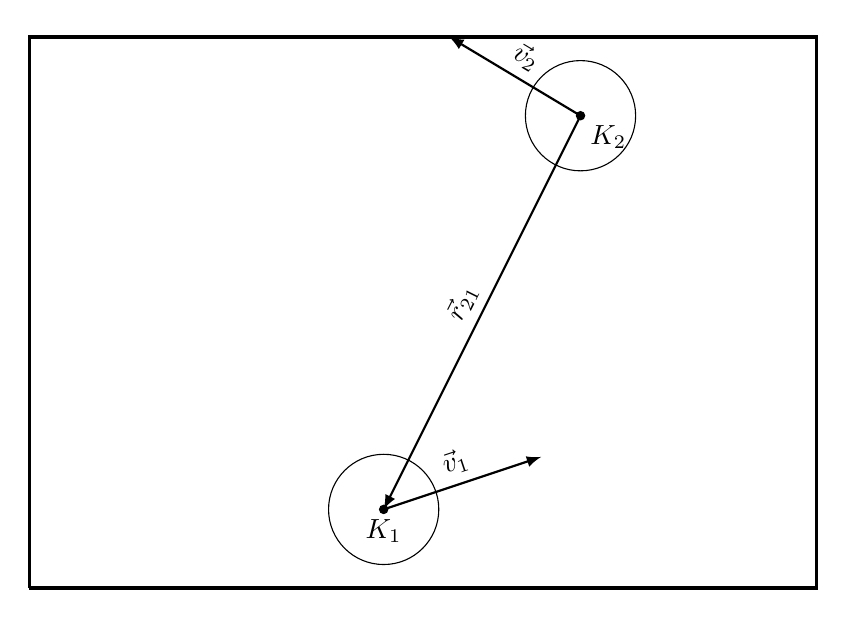
\begin{tikzpicture}
    \coordinate (Origin)   at (0,0);
    \coordinate (OL) at (0,\BoxH);
    \coordinate (OR) at (\BoxW,\BoxH);
    \coordinate (UR) at (\BoxW,0);
    
    \draw [very thick] (Origin) -- (OL) -- (OR) -- (UR) -- (Origin);
    
    \coordinate [label={below right:$K_2$}] (K2) at (\Kx,\Ky);
    \drawKugel{K2};
    
    \coordinate [label={below:$K_1$}] (K1) at (\Kx+\Dx,\Ky+\Dy);
    \drawKugel{K1};

	\draw[-latex, thick] (K2) -- (K1) node[midway,above,sloped] {$\vdis$};
	
	\draw[-latex, thick] (K1) -- (\Kx+\Dx+\vxa, \Ky+\Dy+\vya) node[midway,above,sloped] {$\vec{v}_1$};
	\draw[-latex, thick] (K2) -- (\Kx+\vxb, \Ky+\vyb) node[midway,above,sloped] {$\vec{v}_2$};
  \end{tikzpicture}
  \caption{Ausgansposition der betrachteten Kugeln.}
  \label{fig:Koortrans01}
\end{figure}





Um eine leichter zu handhabende Darstellung zu erhalten und Effekten mit Stoßpartnern am Rand unserer Box aus dem Weg zu gehen transformieren wir unser System so, dass sich eine der am berechneten Stoß beteiligten Kugeln im Zentrum der Box befindet. Da wir eine Box mit periodischen Randbedingungen gewählt haben ist dies ohne weitere Probleme möglich. In \reffig{Koortrans02} ist das Resultat einer solchen Verschiebung um Kugel 2 zu sehen.

% !TeX root = ../Harte_Kugeln.tex

\begin{figure}[H]
  \centering
  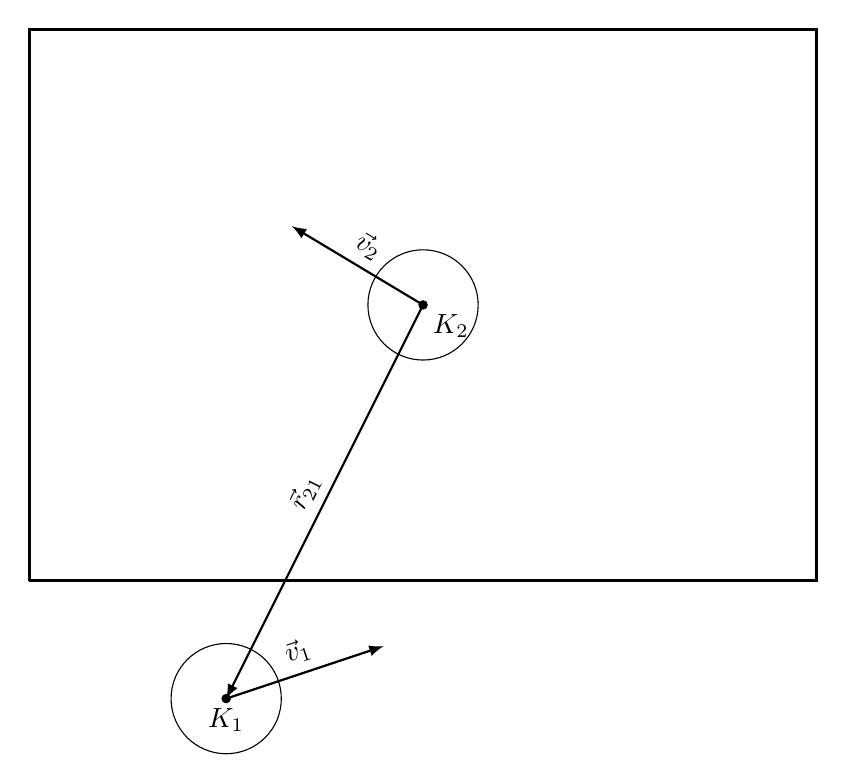
\begin{tikzpicture}
    \coordinate (Origin)   at (0,0);
    \coordinate (OL) at (0,\BoxH);
    \coordinate (OR) at (\BoxW,\BoxH);
    \coordinate (UR) at (\BoxW,0);
    
    \draw [very thick] (Origin) -- (OL) -- (OR) -- (UR) -- (Origin);
    
    \coordinate [label={below right:$K_2$}] (K2) at (\BoxC);
    \drawKugel{K2};
    
    \coordinate [label={below:$K_1$}] (K1) at (\BoxWh+\Dx,\BoxHh+\Dy);
    \drawKugel{K1};
    
	\draw[-latex, thick] (K2) -- (K1) node[midway,above,sloped] {$\vdis$};
	
	\draw[-latex, thick] (K1) -- (\BoxWh+\Dx+\vxa, \BoxHh+\Dy+\vya) node[midway,above,sloped] {$\vec{v}_1$};
	\draw[-latex, thick] (K2) -- (\BoxWh+\vxb, \BoxHh+\vyb) node[midway,above,sloped] {$\vec{v}_2$};
  \end{tikzpicture}
  \caption{Koordinatentransformation Kugel 2 ins Zentrum der Box.}
  \label{fig:Koortrans02}
\end{figure}

Da es durch die Verschiebung dazu kommen kann, dass Kugel 1 die betrachtete Box verlässt, wie in \reffig{Koortrans03} zu sehen, muss sie durch Anwendung der Randbedingungen wieder in die Box gelegt werden.

% !TeX root = ../Harte_Kugeln.tex

\begin{figure}[H]
  \centering
  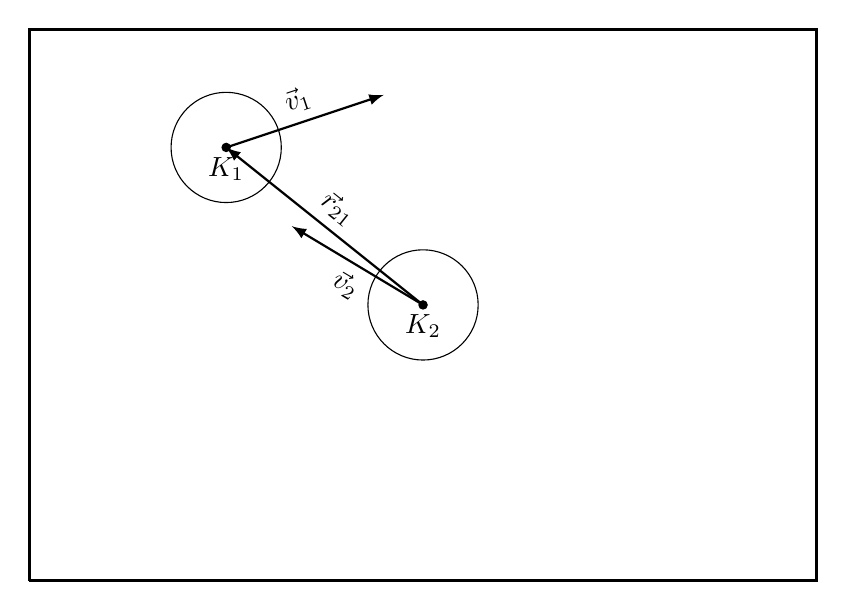
\begin{tikzpicture}
    \coordinate (Origin)   at (0,0);
    \coordinate (OL) at (0,\BoxH);
    \coordinate (OR) at (\BoxW,\BoxH);
    \coordinate (UR) at (\BoxW,0);
    
    \draw [very thick] (Origin) -- (OL) -- (OR) -- (UR) -- (Origin);
    
    \coordinate [label={below:$K_2$}] (K2) at (\BoxC);
    \drawKugel{K2};
    
    \coordinate [label={below:$K_1$}] (K1) at (\BoxWh+\Dx,\BoxHh+\Dy+\BoxH);
    \drawKugel{K1};
    
	\draw[-latex, thick] (K2) -- (K1) node[midway,above,sloped] {$\vdis$};
	
	\draw[-latex, thick] (K1) -- (\BoxWh+\Dx+\vxa, \BoxHh+\Dy+\BoxH+\vya) node[midway,above,sloped] {$\vec{v}_1$};
	\draw[-latex, thick] (K2) -- (\BoxWh+\vxb, \BoxHh+\vyb) node[midway,below,sloped] {$\vec{v}_2$};
  \end{tikzpicture}
  \caption{Kugel 1 wieder in die Box zurück gesetzt.}
  \label{fig:Koortrans03}
\end{figure}

Es ist nur Relativgeschwindigkeit der beiden Kugeln entscheidend und daher kann die Kugel im Zentrum als in Ruhe betrachten, solange sich die andere Kugeln mit der Relativgeschwindigkeit $\vvel=\vec{v}_1-\vec{v}_2$ bewegt.
 
% !TeX root = ../Harte_Kugeln.tex

\begin{figure}[H]
  \centering
  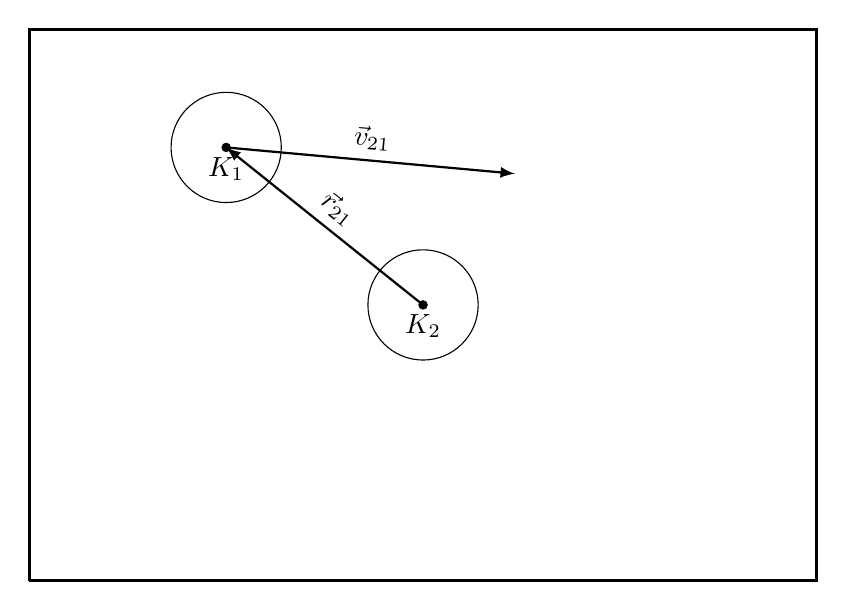
\begin{tikzpicture}
    \coordinate (Origin)   at (0,0);
    \coordinate (OL) at (0,\BoxH);
    \coordinate (OR) at (\BoxW,\BoxH);
    \coordinate (UR) at (\BoxW,0);
    
    \draw [very thick] (Origin) -- (OL) -- (OR) -- (UR) -- (Origin);
    
    \coordinate [label={below:$K_2$}] (K2) at (\BoxC);
    \drawKugel{K2};
    
    \coordinate [label={below:$K_1$}] (K1) at (\BoxWh+\Dx,\BoxHh+\Dy+\BoxH);
    \drawKugel{K1};
    
	\draw[-latex, thick] (K2) -- (K1) node[midway,above,sloped] {$\vdis$};
	
	\draw[-latex, thick] (K1) -- (\BoxWh+\Dx+\vxa-\vxb, \BoxHh+\Dy+\BoxH+\vya-\vyb) node[midway,above,sloped] {$\vvel$};
  \end{tikzpicture}
  \caption{Relativgeschwindigkeit auf Kugeln 1 übertragen.}
  \label{fig:Koortrans04}
\end{figure}

Hat man nun eine Darstellung wie in \reffig{Koortrans04} vorliegen, so kann man die Kollisionszeit durch Anwendung simpler Geometrie erhalten.
Es gilt die Abstandsgleichung 
\begin{equation}
	\vec{x} = \vdis + t\cdot\vvel
\end{equation}
mit 
\begin{equation}
	\left|\vec{x}\right| \overset{!}{=} \dia \Rightarrow \left|x\right|^2 = \dia^2
\end{equation}
zu lösen, wobei $\dia=\sigma_1/2 + \sigma_2/2$ gilt.

Somit erhält man
\begin{align}
	\dia^2	&= \left(\vdis + t\cdot\vvel \right)^2 \\
			&= \vdissq + 2t\cdot\vdis\cdot\vvel + t^2\vvelsq
\end{align}
und nach Auflösen nach der Kollisionszeit $t$
\begin{equation}
	t_{1,2}=\frac{\vdis\cdot\vvel \pm \sqrt{\left(\vdis\cdot\vvel\right)^2 - \vdissq\vvelsq + \vvelsq\dia^2}}{\vvelsq}.
\end{equation}

Die Berechnung kann noch vereinfacht werden. Wie man in \reffig{Koortrans04} sieht, kann es nur zu einer Kollision kommen wenn $\vdis\cdot\vvel < 0$ ist. Daher kann nur die Addition des Wurzelterms zu einem Ergebnis mit positiver Zeit führen.\\
Kommt es zu keinem Stoß in dieser Box, so verlässt Kugel 1 die Box und wird, entsprechend den Randbedingungen des Systems, wieder zurückgesetzt.


\subsubsection{Berechnung der Impulsänderung durch Stöße}
Der Berechnung der Stöße liegt die Erhaltung von Impuls und Energie zugrunde. Wenn zwei Kugeln mit Massen $m_1,m_2$ und Geschwindigkeiten $v_1,v_2$ aufeinandertreffen, verändern sich die Geschwindigkeiten zu $v_1'$ und $v_2'$.
\begin{align*}
m_1v_1 + m_2v_2 &= m_1v_1'+m_2v_2'\\
\frac{m_1v^2_1}{2}+\frac{m_2v^2_2}{2} &= \frac{m_1v'^2_1}{2}+\frac{m_2v'^2_2}{2}
\end{align*}
\\
Da bei einem Stoß nur eine Kraft normal auf die Kugeln (parallel zum Vektor $\vec r_{12} = \vec r_2 - \vec r_1$) zwischen den beiden Kugelmittelpunkten $\vec r_i, i\in \{1,2\}$ wirkt, ist auch nur die entsprechende Komponente der Geschwindigkeit betroffen.\\
Aus den Erhaltungssätzen und dieser Überlegung lässt sich dann das Verhalten der Kugeln bei einem Stoß für den Spezialfall zweier Kugeln identischer Masse herleiten:
\begin{align*}
\vec v_1' &= \vec v_1 + \Delta \vec v\\
\vec v_2'& = \vec v_2 - \Delta \vec v\\
\Delta\vec v &= \left(\vec r_2 - \vec r_1\right) \cdot \left(\vec v_2 - \vec v_1\right)\frac{\left(\vec r_2 - \vec r_1\right)}{R^2}
\end{align*}

\begin{figure}[H] \centering
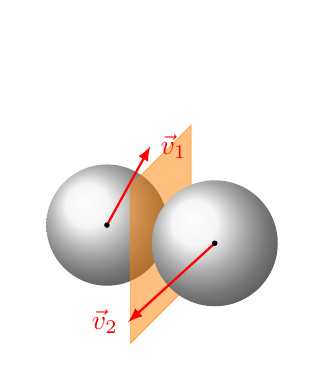
\begin{tikzpicture}
\draw[white] (-1,-1.75) rectangle(2.5,2.5);
  \shade[ball color=gray!10!] (0,0) coordinate(A) circle (0.77) ;
  \draw[orange,fill=orange, opacity=0.5] (0.8,-1,1.3) -- ++(0,2,0) -- ++(0,0,-2) -- ++(0,-2,0) -- cycle;
  \shade[ball color=gray!10!] (1.6,0,0.6) coordinate(B) circle (0.8) ;
  \draw[thick,-latex,red] (A) --+ (0.55,1) node[right]{$\vec v_1$} ;
  \draw[thick,-latex,red] (B) --+ (-1.1,-1) node[left]{$\vec v_2$} ;
%  \draw (4,.2) node[right]{H$^-$} ;
  \foreach \point in {A,B}
  	\fill [black] (\point) circle (1pt) ;
\end{tikzpicture} \hfill
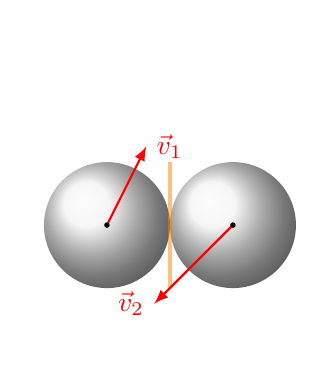
\begin{tikzpicture}
\draw[white] (-1,-1.75) rectangle(2.5,2.5);


  \shade[ball color=gray!10!] (0,0) coordinate(A) circle (0.8) ;
  \shade[ball color=gray!10!] (1.6,0) coordinate(B) circle (0.8) ;
  \draw[very thick, orange, opacity=0.5](0.8,-0.8) --+(0,1.6);
  \draw[thick,-latex,red] (A) --+ (0.5,1) node[right]{$\vec v_1$} ;
  \draw[thick,-latex,red] (B) --+ (-1,-1) node[left]{$\vec v_2$} ;
%  \draw (4,.2) node[right]{H$^-$} ;
  \foreach \point in {A,B}
  	\fill [black] (\point) circle (1pt) ;
\end{tikzpicture} \hfill
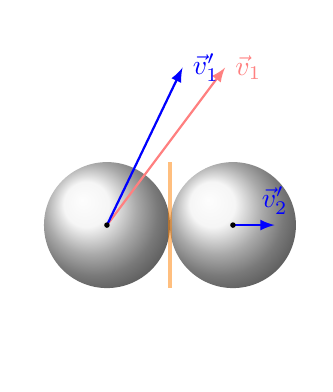
\begin{tikzpicture}
\draw[white] (-1,-1.75) rectangle(2.5,2.5);
  \shade[ball color=gray!10!] (0,0) coordinate(A) circle (0.8) ;
  \shade[ball color=gray!10!] (1.6,0) coordinate(B) circle (0.8) ;
    \draw[very thick, orange, opacity=0.5](0.8,-0.8) --+(0,1.6);
  \draw[thick,-latex,red!50!] (A) --+ (1.5,2) node[right]{$\vec v_1$} ;
  \draw[thick,-latex,blue] (A) --+ (0.96,2) node[right]{$\vec v_1'$} ;
  \draw[thick,-latex,blue] (B) --+ (0.53,0) node[above]{$\vec v_2'$} ;
%  \draw (4,.2) node[right]{H$^-$} ;
  \foreach \point in {A,B}
  	\fill [black] (\point) circle (1pt) ;
\end{tikzpicture} \hfill
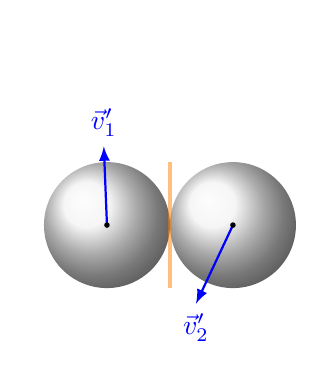
\begin{tikzpicture}
\draw[white] (-1,-1.75) rectangle(2.5,2.5);
  \shade[ball color=gray!10!] (0,0) coordinate(A) circle (0.8) ;
  \shade[ball color=gray!10!] (1.6,0) coordinate(B) circle (0.8) ;
    \draw[very thick, orange, opacity=0.5](0.8,-0.8) --+(0,1.6);
  \draw[thick,-latex,blue] (A) --+ (-0.04,1) node[above]{$\vec v_1'$} ;
  \draw[thick,-latex,blue] (B) --+ (-0.47,-1) node[below]{$\vec v_2'$} ;
%  \draw (4,.2) node[right]{H$^-$} ;
  \foreach \point in {A,B}
  	\fill [black] (\point) circle (1pt) ;
\end{tikzpicture}
\caption{Stoß von 2 Kugeln in 3 Dimensionen (ganz links) kann auf 2 dimensionalen Fall reduziert werden (mitte links), bei dem eine Kugel vor dem Stoß ruht (mitte rechts). Geschwindigkeiten vor dem Stoß jeweils in rot, Geschwindigkeiten der Kugeln nach dem Stoß jeweils in blau }
 \label{fig:kugelnstoss}
\end{figure} 
